\begin{figure}[!h]
\centering
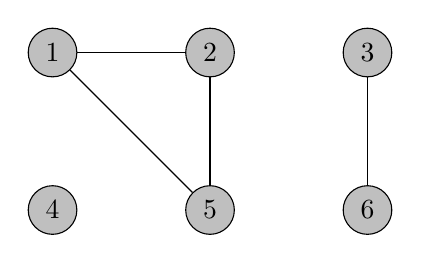
\begin{tikzpicture}[scale=1, vertex/.style = {circle,fill=gray!50,draw}, edge/.style = {-,thin}]
% vertex
\node[vertex] (n4) at (1,1) {4};
\node[vertex] (n5) at (3,1)  {5};
\node[vertex] (n2) at (3,3)  {2};
\node[vertex] (n1) at (1,3)  {1};
\node[vertex] (n6) at (5,1)  {6};
\node[vertex] (n3) at (5,3)  {3};
%edges
\draw[edge] (n1) to (n2);
\draw[edge] (n1) to (n5);
\draw[edge] (n2) to (n5);
\draw[edge] (n3) to (n6);
\end{tikzpicture}
\caption{Grafo no direccionado}
Un grafo no direccionado $G=(V,E)$, donde $V=\{1,2,3,4,5,6\}$ y $E=\{(1,2),(1,5),(2,5),(3,6)\}$.\\Fuente: \cite{Cormen2009}.
\label{grafoNoDir}
\end{figure}
\subsection{Grafo bipartito}
En \cite{Cormen2009} encontramos la siguiente definición. Un grafo bipartito es un grafo no direccionado $G=(V,E)$ en el cual $V$ puede ser particionado en dos conjuntos $V_1$ y $V_2$ talque $(u,v) \in E$ implica que $u \in V_1$ y $v \in V_2$ o $v \in V_1$ y $u \in V_2$. Es decir todas las aristas relacionan los conjuntos $V_1$ y $V_2$, como se muestra en la figura \ref{grafoBip}.
\begin{figure}[!h]
\centering
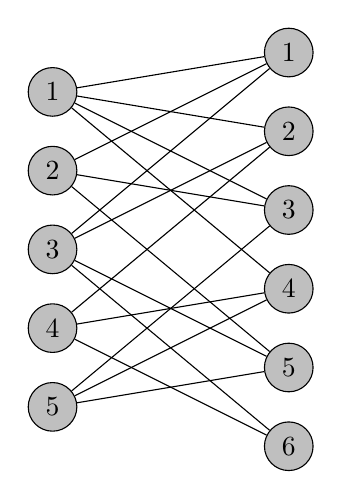
\begin{tikzpicture}[scale=1, vertex/.style = {circle,fill=gray!50,draw}, edge/.style = {-,thin}]
% vertex
\node[vertex] (n1) at (1,5.5) {1};
\node[vertex] (n2) at (1,4.5)  {2};
\node[vertex] (n3) at (1,3.5)  {3};
\node[vertex] (n4) at (1,2.5)  {4};
\node[vertex] (n5) at (1,1.5)  {5};
\node[vertex] (n6) at (4,6)  {1};
\node[vertex] (n7) at (4,5)  {2};
\node[vertex] (n8) at (4,4)  {3};
\node[vertex] (n9) at (4,3)  {4};
\node[vertex] (n10) at (4,2)  {5};
\node[vertex] (n11) at (4,1)  {6};
%edges
\draw[edge] (n1) to (n6);
\draw[edge] (n1) to (n7);
\draw[edge] (n1) to (n8);
\draw[edge] (n1) to (n9);
\draw[edge] (n2) to (n6);
\draw[edge] (n2) to (n8);
\draw[edge] (n2) to (n10);
\draw[edge] (n3) to (n6);
\draw[edge] (n3) to (n7);
\draw[edge] (n3) to (n10);
\draw[edge] (n3) to (n11);
\draw[edge] (n4) to (n7);
\draw[edge] (n4) to (n9);
\draw[edge] (n4) to (n11);
\draw[edge] (n5) to (n8);
\draw[edge] (n5) to (n9);
\draw[edge] (n5) to (n10);
\end{tikzpicture}
\caption{Grafo bipartito}
Un grafo bipartito con un numero impar de vértices.\\Fuente: \cite{Cormen2009}.
\label{grafoBip}
\end{figure}